\section{Implementacja}
\subsection{Narzędzia}
W celu ułatwienia pracy kilku osób nad projektem zostało wykorzystane narzędzie GitHub \cite{github}. Zastosowano również ciągłą integrację wykorzystując Travis CI \cite{travis}. Do automatyzuji budowy oprogramowania na platformę Java użyto Apache Maven \cite{maven}.

\subsection{Środowisko}
Do stworzenia klienta aplikacji użyto środowiska Visual Studio Code. Część serwerowa powstała w~środowisku Eclipse EE z~wykorzystaniem
serwera aplikacyjnego WildFly \cite{wildFly_doc} oraz bazy danych MySQL. Tabele bazy danych zostaną utworzone
przy pierwszym uruchomieniu serwera. Należy skonfigurować serwer WildFly tak, aby mógł korzystać z~baz danych MySQL. 

\subsection{Serwer}
Do zadań serwera należy zarządzanie przechowywanymi informacjami oraz ich
udostępnianie. Został on stworzony w~technologii Java EE. Kod podzielono na warstwy: danych (model), logiki (managery), oraz interfejs wejściowy (REST). Warstwa danych odpowiada za przechowywanie informacji w~bazie danych oraz dostęp do nich. Warstwa logiki realizuje funkcje takie jak np. wgrywanie zdjęcia, czy rejestracja użytkownika. Interfejs REST przyjmuje żądania HTTP, wyodrębnia z~nich dane i~przekazuje je do warstwy logiki. Generując odpowiedź tworzy on odpowiedź HTTP, ustalając dla niej m.in. odpowiedni kod odpowiedzi oraz treść.

\subsubsection{Model}
W celu stworzenia bazy danych przedstawionej w~projekcie aplikacji utworzono
klasy modelowe. Są to zwykłe klasy Javy opatrzone specjalnymi adnotacjami.
Umieszczone one zostały w~pakiecie photoGallery.model. Przykład takiej klasy
przedstawiono na listingu \ref{lst:image}. Za pomocą adnotacji są w
niej tworzone klucze główne (adnotacja @Id oraz @GeneratedValue do
automatycznego generowania wartości) oraz klucze obce (adnotacje @ManytoOne oraz
@JoinColumn). Dodatkowo definiowane są także zapytania,
które będą mogły być później
wykorzystane (@NamedQuery). 

\lstinputlisting[caption={Fragment klasy modelu Image, pominięto metody oraz pola nie posiadające adnotacji}, label=lst:image]
{listings/Image.java}

Do wykonywania operacji na bazie danych wykorzystano klasy DAO. Każda klasa
modelu posiada swoją własną klasę DAO. Klasy te można znaleźć w~pakiecie
photoGallery.dao. Ze względu na to, że wszystkie posiadają podobne funkcje
stworzono abstrakcyjną klasę generyczną GenericDAO. Dostarcza ona podstawowych
operacji takich jak wyszukanie w~bazie obiektu po identyfikatorze, jego
tworzenie, modyfikacja oraz usuwanie, a także pobieranie wszystkich obiektów. Klasa ta została przedstawiona na listingu
\ref{lst:genericDAO}. DAO konkretnej klasy rozszerza generyczne DAO oraz, jeśli
to potrzebne, dodaje dodatkowe metody. Przykład klasy DAO pokazano na listingu \ref{lst:UserDAO}. Rozszerza ona klasę GenericDAO podając typ danych na jakich będzie operowała oraz implementuje metodę GetClassType().

\newpage
\lstinputlisting[caption={Klasa GenericDAO}, label=lst:genericDAO]
{listings/GenericDAO.java}

\lstinputlisting[caption={Klasa UserDAO}, label=lst:UserDAO]
{listings/UserDAO.java}

\subsubsection{\textcolor{red}{Logika aplikacji}}
Logika aplikacji, realizująca jej funkcjonalności po stronie serwera, została umieszczona w~klasach Managerów (znajdującą się one w~pakiecie photoGallery.manager). Są to bezstanowe komponenty sesyjne EJB. Każda ich metoda realizuje jedno polecenie, które jest niezależne od innych. Managery posiadają dostęp do DAO dzięki wstrzykiwaniu zależności (ang. dependency injection). Na listingu
\ref{lst:UserManager} przedstawiono klasę UserManager, która zajmuje się
operacjami na użytkownikach - procesem rejestracji i logowania. Adnotacja w~wierszu pierwszym informuje o~tym, że klasa ta
jest bezstanowym EJB. Wiersze 4-5 odpowiadają za wstrzyknięcie DAO
odpowiedzialnego za operacje na tabeli przechowującej dane użytkowników.
Metoda loginUser() (wiersze 9-21) przyjmuje jako parametry login oraz
hasło użytkownika. Po udanym logowaniu zwracany jest obiekt użytkownika, w
przeciwnym wypadku zgłaszany jest wyjątek logowania. Występuje on w~przypadku
gdy hasło jest niepoprawne, a także gdy nie istnieje użytkownik o~podanym loginie. Proces logowania przebiega następująco:
\begin{itemize}
	\item pobranie użytkownika o~podanym loginie, jeśli nie istnieje zgłoszenie wyjątku (wiersze 10-12),
        \item wygenerowanie hashu z~hasła (wiersz 13. oraz metoda generateHash() w~wierszach 27-42),
	\item porównanie wygenerowanego hashu z~zapisanym w~bazie oraz zgłoszenie wyjątku jeśli nie są identyczne (wiersze 13-16),
	\item wygenerowanie tokena i~zapisanie go w~bazie (wiersze 17-19 oraz metoda generateToken() w~wierszach 23-25),
	\item czyszczenie pola zwierającego hash hasła, modyfikacja ta dotyczy tylko obiektu zwracanego przez funkcje, nie ma wpływu na dane w~bazie danych (wiersz 19.).
\end{itemize}

\lstinputlisting[caption={Klasa UserManager}, label=lst:UserManager]
{listings/UserManager.java}

\subsubsection{\textcolor{red}{Interfejs wejściowy}}
Dostęp do logiki aplikacji został udostępniony poprzez interfejs REST stworzony
przy użyciu standardu JAX-RS. W celu kontroli dostępu do aplikacji
(ochrona przed niezalogowanymi użytkownikami) został utworzony filtr przechwytujący wchodzące zapytania (listing \ref{lst:filter}). 
Pobiera on zawartość nagłówka \textit{AUTHORIZATON}, a następnie, dzięki wstrzykniętemu managerowi użytkowników, decyduje czy żądanie może zostać przepuszczone dalej. W nagłówku znajduje się login użytkownika oraz token wygenerowany w~trakcie procesu logowania. W przypadku, gdy token będzie niepoprawny, żądanie zostanie przerwane z~kodem odpowiedzi \textit{UNAUTHORIZED}.

\lstinputlisting[caption={Klasa LoginFilter}, label=lst:filter]
{listings/LoginFilter.java}

Nie każda metoda jest chroniona przed dostępem niezalogowanych użytkowników. Metody chronione są oznaczone adnotacją, którą jest też oznaczony filtr (adnotacja @Secured przedstawiona na listingu \ref{lst:securedAnnotation}).

\lstinputlisting[caption={Adnotacja @Secured}, label=lst:securedAnnotation]
{listings/Secured.java}

Na listingu \ref{lst:ImageRestEndpoint} został przedstawiony fragment klasy będącej punktem wejścia do serwera odpowiedzialnym za zdjęcia. Za pomocą adnotacji oznaczono ścieżkę oraz typ danych, które przyjmują oraz zwracają metody danej klasy. Dodatkowo każda metoda jest opatrzona adnotacją z~konkretną ścieżką oraz z~metodą HTTP jaką obsługuje. Każda metoda zwraca obiekt typu Response, który reprezentuje odpowiedź HTTP. Poprzez ten obiekt ustawiany jest kod odpowiedzi oraz jej treść w~formacie JSON.

\lstinputlisting[caption={Fragment klasy ImageRestEndpoint}, label=lst:ImageRestEndpoint]
{listings/ImageRestEndpoint.java}

\subsection{\textcolor{red}{Klient}}
Aplikacja kliencka została wykonana...


\subsubsection{Połączenie z~serwerem}
Komunikacja z~serwerem w~całości realizowana jest poprzez protokół HTTP. 

Całość
komunikacji zawarta została w~klasie RestClient. Posiada ona metodę
odpowiedzialną za tworzenie połączenia (listing \ref{lst:getConnection}) oraz
metody realizujące konkretne zadania, takie jak utworzenie wycieczki, czy
aktualizację informacji o~użytkowniku na serwerze. Przebieg realizacji pojedynczego zadania po stronie klienta przedstawiono na rysunku \ref{fig:clientRequest}. Większość metod może zakończyć się na 3 sposoby:
\begin{itemize}
	\item operacja wykonana pomyślnie, zwrócona oczekiwana wartość,
	\item operacja się nie powiodła, zwrócona zostaje wartość \texttt{null} (w przypadku gdy wystąpi nieoczekiwany błąd po stronie serwera. Dzięki temu, gdy niepowodzenie nie wpływa na działanie aplikacji, użytkownik nie będzie o~tym poinformowany) lub komunikat błędu,
	\item nastąpił błąd połączenia, zgłoszony zostaje wyjątek.
\end{itemize}

Do konwersji obiektów Javy na format JSON i~odwrotnie użyto biblioteki Jackson.
Udostępnia ona klasę ObjectMapper, która posiada metody umożliwiające taką konwersje. Przykład użycia przedstawiono na listingu \ref{lst:objectMapper}.

\lstinputlisting[caption={Przykład użycia obiektu ObjectMapper}, label=lst:objectMapper]
{listings/Image.java}

\lstinputlisting[caption={Metoda przygotowująca nagłówek zapytania HTTP}, label=lst:getConnection]
{listings/Image.java}

\begin{figure}[ht]
	\centering
	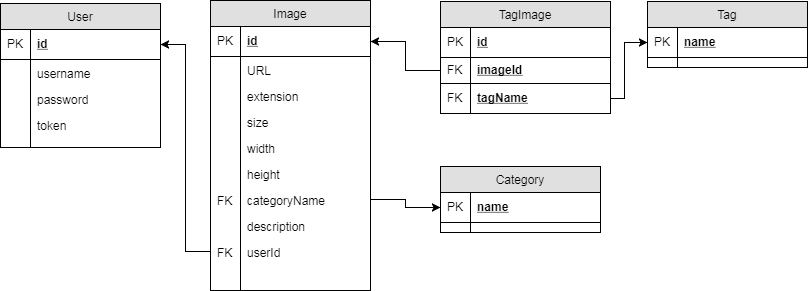
\includegraphics[width = 15cm]{images/bazaDanych}
	\caption{Schemat generowania zapytania po stronie klienta
		\newline Źródło: opracowanie własne}
	\label{fig:clientRequest}
\end{figure}

System Android zabrania wykonywania operacji korzystających z~sieci w~wątku
głównym aplikacji. W~związku z~tym metody klasy RestClient są wywoływane z~klas
dziedziczących po klasie AsyncTask. Dzięki temu komunikacja z~serwerem odbywa
się w~tle, nie blokując interfejsu graficznego. Dodatkowo została utworzona
klasa WaitingAsyncTask dziedzicząca po klasie AsyncTask. Zawiera
ona kod odpowiedzialny za wyświetlanie ikony ładowania informującą użytkownika, że właśnie przeprowadzana jest jakaś operacja. Klasa ta wykorzystywana jest, gdy aplikacja kliencka oczekuje na odpowiedź serwera. Efekt widoczny dla użytkownika pokazano na rysunku \ref{fig:waitingTask}.

\begin{figure}[ht]
	\centering
	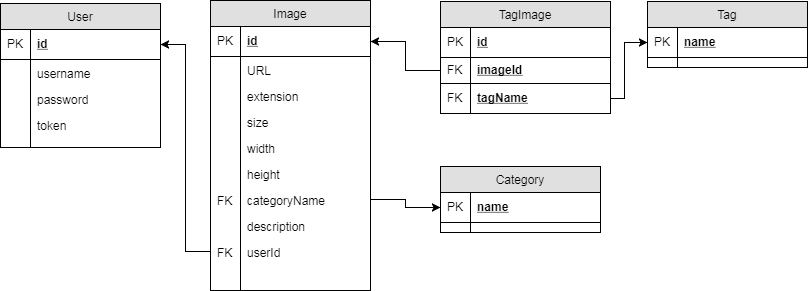
\includegraphics[width = 6cm]{images/bazaDanych}
	\caption{Ekranu oczekiwania na wynik operacji wykonującej się w~tle	\newline Źródło: opracowanie własne}
	\label{fig:waitingTask}
\end{figure}

\subsubsection{Śledzenie pozycji}
Aby móc śledzić aktualną pozycję użytkownika utworzono klasę
GPSListener implementującą interfejs LocationListener. Jest ona rejestrowana
jako obserwator zdarzeń dotyczących systemu GPS. Informacje o~postępach
użytkownika są przechowywane w~klasie UserTripManager (której ważniejsze metody
wypisano na listingu \ref{lst:userTripManager}). Zawiera ona metody
odpowiedzialne za aktualizowanie pozycji użytkownika, obliczanie przebytej
drogi, prędkości średniej oraz chwilowej. W~chwili otrzymania z~systemu GPS
nowej lokalizacji wywoływana jest metoda onLocationChange() (przedstawiona na
listingu \ref{lst:onLocationChange}). Wywoływane są w~niej metody odpowiedzialne
za zaktualizowanie pozycji użytkownika na mapie oraz aktualizacje postępów.
Dodatkowo sprawdzany jest czas od wysłania ostatniej aktualizacji do serwera.
Jeśli upłynął ustalony okres, to aktualizacja zostanie
 wysłana.

\lstinputlisting[caption={Metoda onLocationChange klasy GPSListener}, label=lst:onLocationChange]
{listings/Image.java}

\lstinputlisting[caption={Nagłówki ważniejszych metod klasy UserTripManager}, label=lst:userTripManager]
{listings/Image.java}

Metoda updateLocation() klasy UserTripManager odświeża aktualnie przechowywaną pozycje oraz przebyty dystans. Przewidywany pozostały czas zwracany jest w~minutach, prędkości (chwilowa i~średnia) w~km/h, a dystans w~kilometrach. Zarówno przebyty dystans, jak i~prędkości obliczane są na podstawie pozycji uzyskanych z~systemu GPS.


\subsubsection{Interfejs graficzny}
Interfejs graficzny stworzono wykorzystując powiązane ze sobą aktywności. Po
uruchomieniu aplikacji, jeśli użytkownik nie był wcześniej zalogowany, ukaże się
ekran logowania (rysunek \ref{fig:login}). Po zalogowaniu użytkownik uzyska
dostęp do menu głównego (rysunek \ref{fig:menu}). Pod przyciskiem "Opcje"
dostępne są ustawienia dotyczące rodzaju map oraz częstotliwości komunikowania
się z~serwerem (rysunek \ref{fig:settings}). Ekrany tworzenia wycieczki,
dołączania do niej oraz podglądu trwającej aktualnie wycieczki wykorzystują
zakładki w~celu podziału widoku. Ekran tworzenia wycieczki podzielono na mapę na
której można dodać do niej punkty kontrolne (rysunek \ref{fig:create:1}) oraz
szczegóły, gdzie należy ustalić m.in. nazwę i~opis wycieczki (rysunek
\ref{fig:create:2}). Dołączając do wycieczki trzeba wybrać ją z~listy
(rysunek \ref{fig:list}), a następnie można podejrzeć jej szczegóły oraz
przebieg na mapie. Po dołączeniu do wycieczki, pod opcją "Aktualna wycieczka" będzie dostępna podobna mapa, na której dodatkowo zaznaczeni są uczestnicy
wycieczki. Ponadto, znajdują się tam także zakładki z~wynikami użytkownika, listą innych
uczestników wraz z~ich prędkością (rysunek \ref{fig:tripParticipants}) oraz
z~rozmowami z~innymi uczestnikami. Po wybraniu uczestnika na liście można spróbować wysłać do niego wiadomość (rysunek \ref{fig:chat}). 
Zakładki można zmienić za pomocą gestów przesunięcia (w~prawo lub lewo). W tym celu stworzono abstrakcyjną klasę SlideTabActivity. Zawiera ona kod inicjujący detektor gestów oraz metody odpowiedzialne za reakcje na wybrane gesty. Rozszerzając taką klasę należy przypisać odpowiednie wartości do pól tabNumber i~currentTab. Dodatkowo należy też w~klasach odpowiadających za same zakładki w~metodzie onResume() ustawić pole currentTab. Jest to wymagane gdy do zmiany ekranów wykorzystuje się zarówno gesty, jak i~zakładki.


\lstinputlisting[caption={Klasa SwipeTabActivity}, label=lst:swipe]
{listings/Image.java}

\begin{figure}[ht]	
	\begin{tabular}{ccc}
		\subfloat[Ekran logowania \label{fig:login}]
		{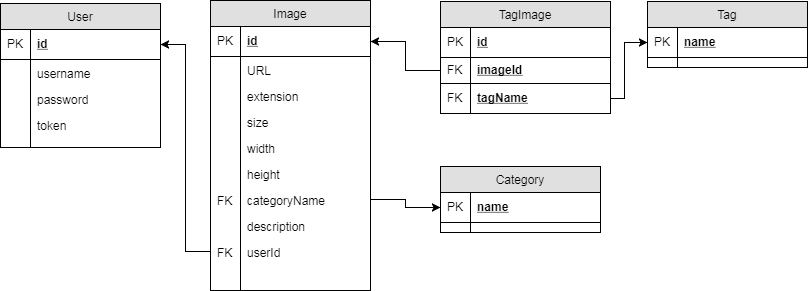
\includegraphics[width = 4.5cm]{images/bazaDanych}} &
		\subfloat[Ekran menu \label{fig:menu}]
		{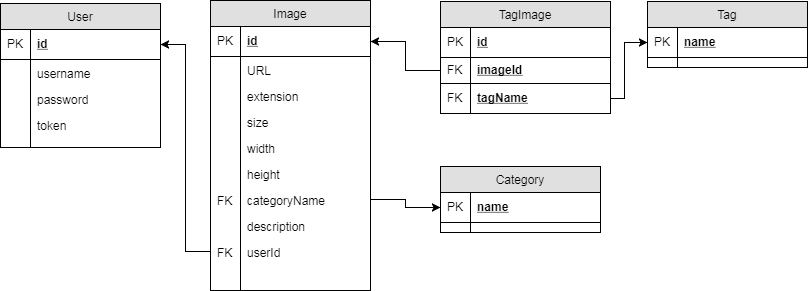
\includegraphics[width = 4.5cm]{images/bazaDanych}} &
		\subfloat[Ekran ustawień \label{fig:settings}]
		{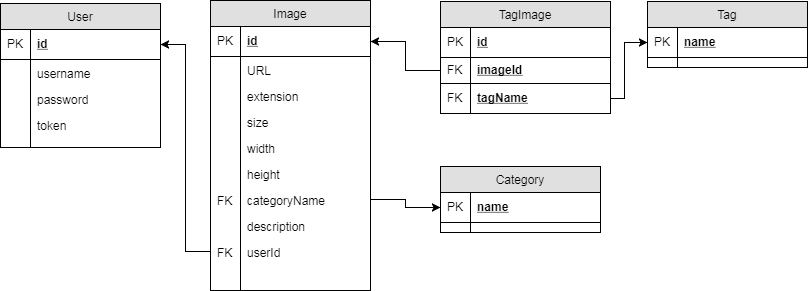
\includegraphics[width = 4.5cm]{images/bazaDanych}}
	\end{tabular}
	\caption{Interfejs graficzny
		\newline Źródło: opracowanie własne}
\end{figure}



\begin{figure}[ht]	
	\begin{tabular}{ccc}
		\subfloat[Tworzenie wycieczki - mapa\label{fig:create:1}]
		{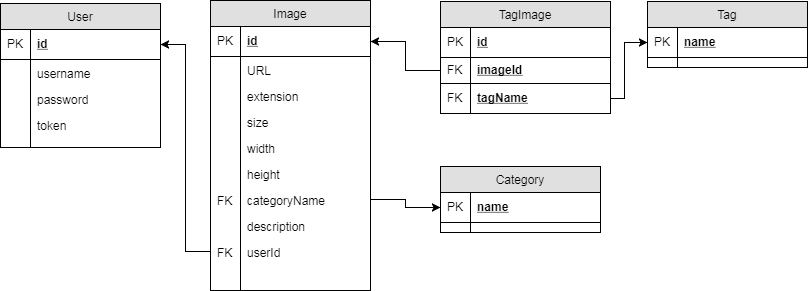
\includegraphics[width = 4.5cm]{images/bazaDanych}} &
		\subfloat[Tworzenie wycieczki - szczegóły\label{fig:create:2}]
		{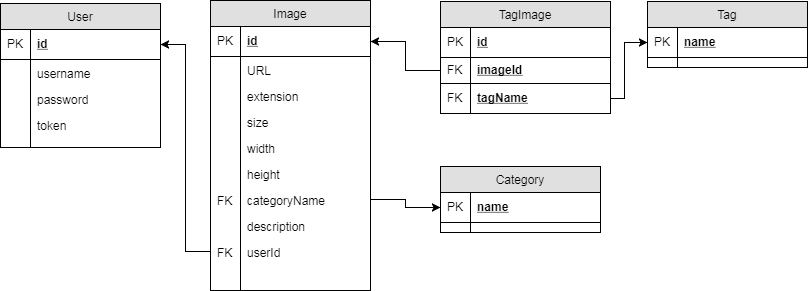
\includegraphics[width = 4.5cm]{images/bazaDanych}} &
		\subfloat[Dołączanie do wycieczki - lista\label{fig:list}]
		{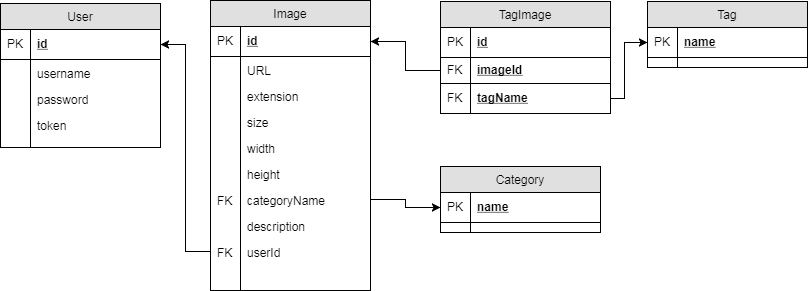
\includegraphics[width = 4.5cm]{images/bazaDanych}}
	\end{tabular}
	\caption{Ekrany tworzenia oraz dołączania do wycieczki
		\newline Źródło: opracowanie własne}
\end{figure}

\begin{figure}[ht]	
	\begin{tabular}{ccc}
		\subfloat[Nasze wyniki\label{fig:tripDetails}]
		{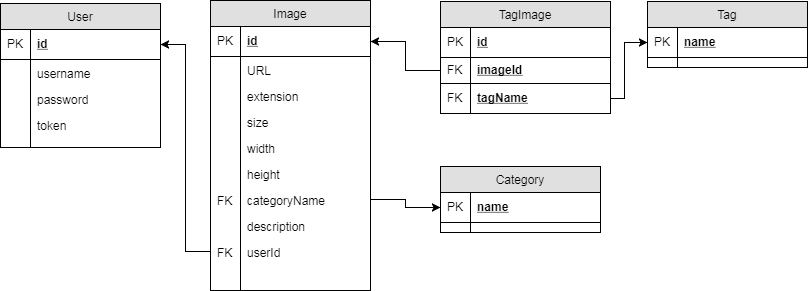
\includegraphics[width = 4.5cm]{images/bazaDanych}} &
		\subfloat[Uczestnicy wycieczki\label{fig:tripParticipants}]
		{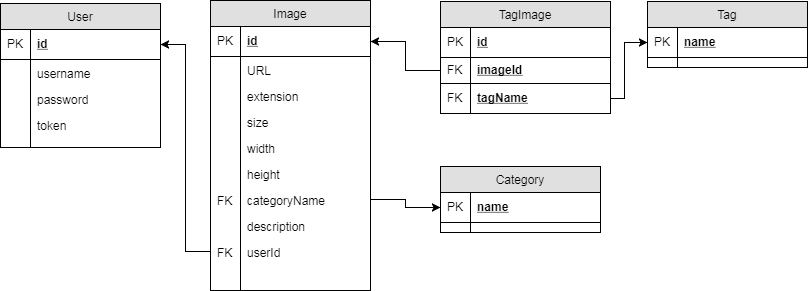
\includegraphics[width = 4.5cm]{images/bazaDanych}} &
		\subfloat[Ekran rozmowy z~innym uczestnikiem \label{fig:chat}]
		{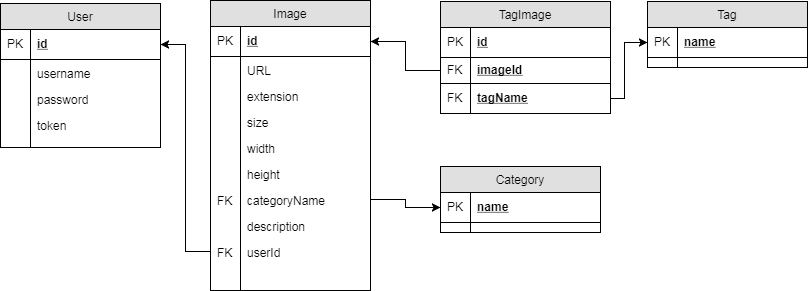
\includegraphics[width = 4.5cm]{images/bazaDanych}}
	\end{tabular}
	\caption{Interfejs graficzny
		\newline Źródło: opracowanie własne}
\end{figure}
